% !TEX root =  ../main_manuscript.tex
\section{Joint Model for Time-to-Event and Longitudinal Data}
\label{sec:jm_framework}
In this appendix section, we provide a short introduction of the PRIAS dataset, and present the joint modeling framework and the corresponding parameter estimation using the Bayesian approach. The PRIAS dataset consists of 5270 AS patients. For each patient, prostate-specific antigen (PSA) measurements (ng/mL) are scheduled every 3 months for first 2 years and every 6 months thereafter. The digital rectal examination (DRE) measurements which are binary with two levels, namely $\mbox{DRE} > \mbox{T1c}$ and $\mbox{DRE} \leq \mbox{T1c}$ \citep{schroder1992tnm}, are scheduled every 6 months. Larger values for PSA and/or larger score for DRE, may indicate cancer progression. Biopsies are scheduled at following fixed follow-up times (measured since inclusion in AS): year 1, 4, 7, and 10, and every 5 years thereafter. An annual schedule is prescribed to those patient's who have a PSA doubling time between 0 and 10 years. PSA doubling time is measured as the inverse of the slope of the regression line through the base two logarithm of the observed PSA values.

Let $T_i^*$ denote the true cancer progression time for the $i$-th AS patient. Let $T_i^R$ and $T_i^{R-1}$ denote the time of his latest and second latest biopsies, respectively. Since biopsies are conducted periodically, $T_i^*$ cannot be observed directly and it is only known to fall in an interval $l_i < T_i^* \leq r_i$, where $l_i = T_i^{R-1}, r_i = T_i^R$ if progression is observed at the latest biopsy, and $l_i = T_i^R, r_i=\infty$ if progression is not observed yet. Further let $\boldsymbol{y}_{1i}, \boldsymbol{y}_{2i}$ denote the $n_{1i} \times 1$ and $n_{2i} \times 1$ vectors of the DRE and PSA longitudinal measurements, respectively. For a sample of $n$ patients the observed data is denoted by $\mathcal{D}_n = \{l_i, r_i, \boldsymbol{y}_{1i}, \boldsymbol{y}_{2i}; i = 1, \ldots, n\}$.
\begin{figure}[!htb]
\captionsetup{justification=justified}
\centerline{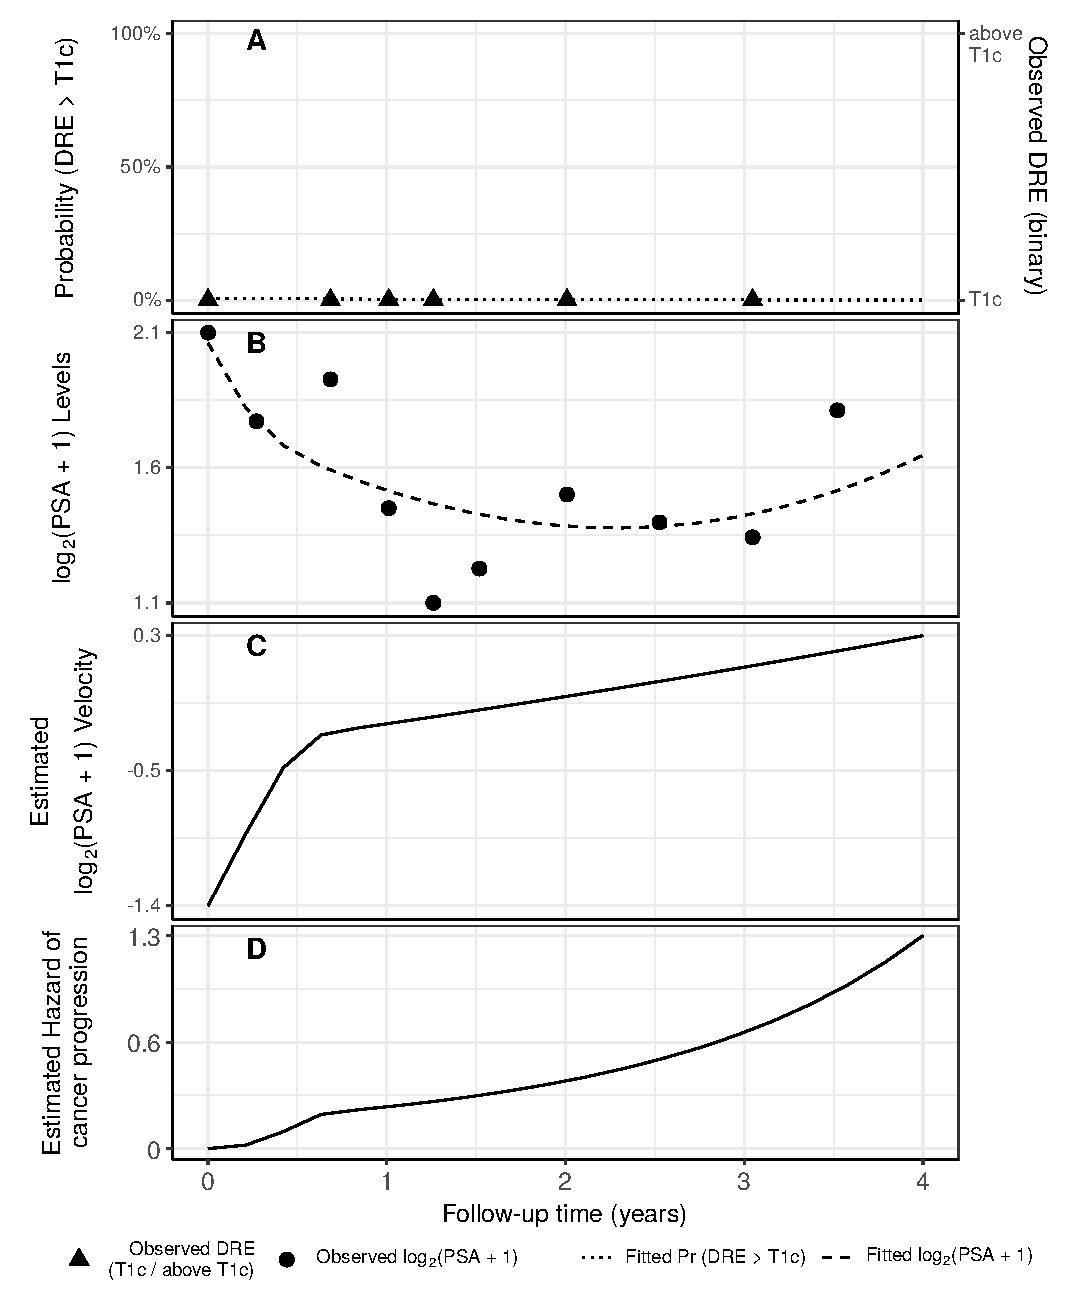
\includegraphics[width=\columnwidth]{images/jmExplanationPlot_1757.eps}}
\caption{Illustration of the joint model fitted to the PRIAS dataset. Panel A shows the fitted $\log_2 \{y_{2i}(t) + 1\}$ velocity (velocity can only be estimated, not observed) over time. Panel B shows the observed and fitted $\log_2 \{y_{2i}(t) + 1\}$ levels. Panel C shows the observed DRE scores and the fitted probability of obtaining a DRE score greater than T1c level. The hazard function shown in Panel D, depends on the fitted log odds of having $\mbox{DRE} > \mbox{T1c}$, and the fitted $\log_2 \{y_{2i}(t) + 1\}$ value and velocity.}
\label{fig:jmExplanationPlot_1757}
\end{figure}

The patient-specific PSA and DRE measurements over time are modeled using a generalized linear mixed effects model. For the $i$-th patient, the sub-model for DRE is given by:
\begin{equation}
\label{eq:long_model_dre}
\begin{aligned}
    \mbox{logit} \big[\mbox{Pr}\{y_{1i}(t) > \mbox{T1c}\}\big] &= \beta_{01} + b_{01i} + (\beta_{11} + b_{11i}) t\\
    &+ \beta_{21} (\mbox{Age}_i-70) + \beta_{31} (\mbox{Age}_i-70)^2\\ 
    \end{aligned}
\end{equation}
where, $\mbox{Age}_i$ is the age of the $i$-th patient at the time of inclusion in AS, $\beta_{\cdot1}$ are the fixed effect parameters, and $b_{\cdot1i}$ are the random effect parameters. An example model fit for DRE is shown in Panel C of Figure \ref{fig:jmExplanationPlot_1757}. For the $i$-th patient, the sub-model for PSA is given by:
\begin{equation}
\label{eq:long_model_psa}
\begin{aligned}
    \log_2 \big\{y_{2i}(t) + 1\big\} &= \beta_{02} + b_{02i} + \sum_{k=1}^4 (\beta_{k2} + b_{k2i})  B_k(t,\mathcal{K})\\ 
    &+ \beta_{52} (\mbox{Age}_i-70) + \beta_{62} (\mbox{Age}_i-70)^2 + \varepsilon_{2i}(t),
    \end{aligned}
\end{equation}
where, $B_k(t, \mathcal{K})$ denotes the $k$-th basis function of a B-spline with three internal knots at $\mathcal{K} = \{0.1, 0.7, 4\}$ years, and boundary knots at 0 and 5.42 years (0.95 quantile of the observed follow-up times). The fixed effects parameters are denoted by $\beta_{\cdot2}$ and random effects are denoted by $b_{\cdot2i}$. The error $\varepsilon_{2i}(t)$ is assumed to be t-distributed with three degrees of freedom and scale $\sigma$ (see Web Appendix C.1), and is independent of the random effects $b_{\cdot2i}$. An example model fit for PSA is shown in Panel B of Figure \ref{fig:jmExplanationPlot_1757}. To account for the association between the DRE and PSA measurements, we link their corresponding random effects. More specifically, the complete vector of random effects $\boldsymbol{b}_i = (b_{\cdot1i}, b_{\cdot2i})^T$ is assumed to follow a multivariate normal distribution with mean zero and $q\times q$ variance-covariance matrix $\boldsymbol{D}$.

To model the impact of DRE and PSA measurements on the risk of cancer progression, we use a relative risk sub-model. More specifically, the hazard of cancer progression $h_i(t)$ at a time $t$ is given by:
\begin{equation}
\label{eq:rel_risk_model}
\begin{aligned}
    h_i(t) &= h_0(t) \exp\Big(\alpha_{11} \mbox{logit} \big[\mbox{Pr}\{y_{1i}(t) > \mbox{T1c}\}\big]\\
    &+ \alpha_{21} E\big[\log_2 \big\{y_{2i}(t) + 1\big\}\big] + \alpha_{22} \frac{\mathrm{d}{E\big[\log_2 \big\{y_{2i}(t) + 1\big\}\big]}}{\mathrm{d}{t}}\\
    &+ \gamma_1 (\mbox{Age}_i-70) + \gamma_2 (\mbox{Age}_i-70)^2 \Big),
    \end{aligned}
\end{equation}
where, $\gamma_1$, $\gamma_2$ are the coefficients for the effect of Age. The parameter $\alpha_{11}$models the impact of log odds of having $\mbox{DRE} > \mbox{T1c}$ on the hazard of cancer progression. The impact of PSA on cancer progression is modeled in two ways, namely at any time $t$ the effect of the instantaneous underlying value (dashed line in panel B of Figure  \ref{fig:jmExplanationPlot_1757}) of PSA $E[\log_2 \{y_{2i}(t) + 1\}]$ is given by $\alpha_{21}$, and the effect of the instantaneous underlying velocity (panel A in Figure \ref{fig:jmExplanationPlot_1757}) of PSA $\mathrm{d}{E[\log_2 \{y_{2i}(t) + 1\}]}/\mathrm{d}{t}$ is given by $\alpha_{22}$. Lastly, $h_0(t)$ is the baseline hazard at time t, and is modeled flexibly using P-splines \citep{eilers1996flexible}. More specifically:
\begin{equation*}
\log{h_0(t)} = \gamma_{h_0,0} + \sum_{q=1}^Q \gamma_{h_0,q} B_q(t, \boldsymbol{v}),
\end{equation*}
where $B_q(t, \boldsymbol{v})$ denotes the $q$-th basis function of a B-spline with knots $\boldsymbol{v} = v_1, \ldots, v_Q$ and vector of spline coefficients $\gamma_{h_0}$. To avoid choosing the number and position of knots in the spline, a relatively high number of knots (e.g., 15 to 20) are chosen and the corresponding B-spline regression coefficients $\gamma_{h_0}$ are penalized using a differences penalty \citep{eilers1996flexible}. An example fitted hazard is shown in Panel D of Figure \ref{fig:jmExplanationPlot_1757}.  

\subsection{Parameter Estimation}
We estimate parameters of the joint model using Markov chain Monte Carlo (MCMC) methods under the Bayesian framework. Let $\boldsymbol{\theta}$ denote the vector of the parameters of the joint model. The joint model postulates that given the random effects, the time to cancer progression, and the PSA and DRE measurements taken over time are all mutually independent. Under this assumption the posterior distribution of the parameters is given by:
\begin{align*}
p(\boldsymbol{\theta}, \boldsymbol{b} \mid \mathcal{D}_n) & \propto \prod_{i=1}^n p(l_i, r_i, \boldsymbol{y}_{1i}, \boldsymbol{y}_{2i}, \mid \boldsymbol{b}_i, \boldsymbol{\theta}) p(\boldsymbol{b}_i \mid \boldsymbol{\theta}) p(\boldsymbol{\theta})\\
& \propto \prod_{i=1}^n p(l_i, r_i \mid \boldsymbol{b}_i, \boldsymbol{\theta}) p(\boldsymbol{y}_{1i} \mid \boldsymbol{b}_i, \boldsymbol{\theta}) p(\boldsymbol{y}_{2i} \mid \boldsymbol{b}_i, \boldsymbol{\theta}) p(\boldsymbol{b}_i \mid \boldsymbol{\theta}) p(\boldsymbol{\theta}),\\
p(\boldsymbol{b}_i \mid \boldsymbol{\theta}) &= \frac{1}{\sqrt{(2 \pi)^q \text{det}(\boldsymbol{D})}} \exp(\boldsymbol{b}_i^T \boldsymbol{D}^{-1} \boldsymbol{b}_i),
\end{align*}
where the likelihood contribution of the DRE outcome, conditional on the random effects is:
\begin{equation*}
p(\boldsymbol{y}_{1i} \mid \boldsymbol{b}_i, \boldsymbol{\theta}) = \prod_{k=1}^{n_{1i}} \frac{\exp\Big[-\mbox{logit} \big\{\mbox{Pr}(y_{1ik} > \mbox{T1c})\big\} I(y_{1ik}=\mbox{T1c}) \Big]}  {1+\exp\Big[-\mbox{logit} \big\{\mbox{Pr}(y_{1ik} > \mbox{T1c})\big\}\Big]},
\end{equation*}
where $I(\cdot)$ is an indicator function which takes the value 1 if the $k$-th repeated DRE score is T1c, and takes the value 0 otherwise. The likelihood contribution of the PSA outcome, conditional on the random effects is:
\begin{equation*}
p(\boldsymbol{y}_{2i} \mid \boldsymbol{b}_i, \boldsymbol{\theta}) = \frac{1}{\big(\sqrt{2 \pi \sigma^2}\big)^{n_{2i}}} \exp\bigg(-\frac{{\lVert{\boldsymbol{y}_{2i} - \boldsymbol{m}_{2i}}\rVert}^2}{\sigma^2}\bigg),
\end{equation*}
where $\boldsymbol{m}_{2i}$ is the vector of underlying measurement error free values of $\log_2(\boldsymbol{y}_i + 1)$. The latter is given by the sum of the terms without the error term $\boldsymbol{\varepsilon}_{2i}$ in the right hand side of the Equation (\ref{eq:long_model_psa}). The likelihood contribution of the time to cancer progression outcome is given by:
\begin{equation}
\label{web_eq : likelihood_contribution_survival}
p(l_i,r_i\mid \boldsymbol{b}_i,\boldsymbol{\theta}) = \exp\Big\{-\int_0^{l_i} h_i(s)\mathrm{d}{s}\Big\} - \exp\Big\{-\int_0^{r_i}h_i(s)\mathrm{d}{s}\Big\}.
\end{equation}
The integral in (\ref{web_eq : likelihood_contribution_survival}) does not have a closed-form solution, and therefore we use a 15-point Gauss-Kronrod quadrature rule to approximate it.

We use independent normal priors with zero mean and variance 100 for the fixed effects $\boldsymbol{\beta}$, and inverse Gamma prior with shape and rate both equal to 0.01 for the parameter $\sigma^2$. For the variance-covariance matrix $\boldsymbol{D}$ of the random effects we take inverse Wishart prior with an identity scale matrix and degrees of freedom equal to $q$ (number of random effects). For the relative risk model's parameters $\boldsymbol{\gamma}$ and the association parameters $\boldsymbol{\alpha}$, we use independent normal priors with zero mean and variance 100.